\chapter{Экспериментальные результаты}
\label{chapter_experiment}

Предлагаемый метод был реализован в виде программной системы на языке \textit{Java} и протестирован.

\section{Реализация}

При реализации предлагаемого метода были реализованы следующие программные компоненты:
\begin{itemize}
\item Обертка для URL-адреса;
\item Менеджер хоста;
\item Модуль вежливости;
\item Правило;
\item Планировщик;
\item Задание;
\item Загрузчик веб-страниц;
\item Обработчик содержимого страницы;
\item Модули назначения приоритетов:
\begin{itemize}
\item Стратегия обхода в ширину;
\item Использующий нейронную сеть;
\item Использующиуй нейронную сеть и свойства веб-графа;
\end{itemize}
\item Контроллер приоритезации, использующей нейронную сеть;
\item Компонент для извлечения особенностей URL-адреса страницы;
\item Компонент, содержащий нейронную сеть;
\item Словарный модуль;
\item Менеджер коллекции.
\end{itemize}

Основным объектом, с которым происходит работа в программе, является обертка для URL-адреса. Она реализована классом \textit{WebURL}. Каждый экземпляр такого класса содержит мета-информацию о веб-странице, ее $QRank$, время последнего посещения, предполагаемый период обновления, ссылку на менеджер хоста и т.д.

Менеджер хоста  реализован классом \textit{HostController} и предназначен для выполнения правил вежливости для определенного хоста. В каждый момент времени с хостом должно быть установлено только одно соединение. Это реализовано за счет синхронизирования загрузок веб-страницы с одного хоста посредством использования поля \textit{lock} менеджера хоста, являющегося экземпляром класса \textit{Lock}. Кроме того, экземляр класса хранит на модуль вежливости, который определяет правила доступа к страницам хоста. Также менеджер хранит количество страниц с текущего хоста, имеющихся в коллекции.

Модуль вежливости предназначен для соблюдения правил вежливости, описанных в файле \textit{robots.txt}, содержащемуся в корневом каталоге многих сайтов. Модуль вежливости реализован классом \textit{PolitenessModule}, содержащий множество (экземляр класса \textit{TreeSet}) правил, являющихся экземплярами класса \textit{Rule}. Правило хранит текстовый шаблон (\textit{Pattern}), удовлетворяющий набору каталогов сайта, и правило доступа (доступно или нет). Порядок на множестве введен для быстрого определения доступности того или иного URL-адреса.

Планировщик реализован классом \textit{Scheduler}. Планировщик на каждом шаге цикла основного этапа алгоритма формирует $K$ заданий, являющихся экземплярами исполняемого (\textit{Runnuble}) класса \textit{PageProceccingTask}. Эти задания передаются исполнителю (экземпляр класса \textit{ExecutorService}). Задание состоит из следующих инструкций для последовательной обработки. Загрузка, осуществляемая загрузчиком веб-страниц. Обработка содержимого и извлечение ссылок со страницы, осуществляемые обаботчиком содержимого страницы. И наконец отправка менеджеру коллекции для дальнейшей обработки. Обработка заданий осуществляется в несколько потоков.

Модуль назначения приоритетов является экземпляром класса, наследующего абстрактный класс \textit{PrioritizationModule}. Разработаны два метода приоритезации: первый использует только нейронную сеть, а второй --- нейронную сеть и анализ веб-графа. Реализованы они соотвественно классами \textit{NeuralPrioritizationModule} \textit{NeuralGraphPrioritizationModule}, исходный код которых приведен в приложениях: \ref{code_1} и \ref{code_2}. Кроме того, были реализованы методы приоритезации: \textit{breadth-first}, реализующий стратегию отбора методом обхода в ширину, и \textit{Random},  для сравнения с разработанными стратегиями приоритезации.

Компонент для извлечения особенностей URL-адреса реализован классом \textit{FeaturesExtractor}. Исходный программный код класса приведен в приложении \ref{code_3}. Для каждой из особенностей адреса компонент реализует его численное представление в интервале от $0$ до $1$ посредством нормировки. Для извлечения словарных особенностей термов конструируется словарный модуль, использующий слова английского и русского языков. Причем слова русского языка были заменены на их транслитерационный вид.

Нейронная сеть была реализована с использованием библиотеки \textit{Encog} \cite{encog}. Сеть содержит три слоя нейронов. Входной слой содержит число нейронов, соответствующее числу особенностей URL-адреса веб-страницы (максимальное число особенностей --- $16$). Слой имеет сигмоидную активирующую функцию. Число нейронов в скрытом слое зависит от числа нейронов входного слоя. А именно --- число нейронов скрытого слоя в три раза больше. Скрытый слой так же имеет сигмоидную активирующую функцию. Выходной слой содержит один нейрон и сигмоидную активирующую функцию. Для обучения использовался метод быстрого распространения (\textit{Quickprop}), являющийся улучшением метода обратного распространения ошибки. Подробно он описан в статье \cite{Fahlman88anempirical}. Данная конфигурация сети была подобрана в ходе тестирования на множестве URL-адресов веб-страниц с известными $PageRank$, полученными с использованием \textit{google toolbar}. Именно с такими параметрами отклонение вычисленного ранга от реального $PageRank$ было минимальным.

Менеджер коллекции реализован классом \textit{CollectionHandler}. Он содержит ссылку на модуль приоритезации, посредством которого вычисляются ранги для URL-адресов веб-страниц, передаваемых в коллекцию. Коллекция представлена экзампляром класса \textit{ConcurrentHashMap}, где ключом является строка, а значением --- \textit{WebURL}. Выбрана потоко-безопасная реализация ассоциативного массива, поскольку добавление адресов происходит в несколько потоков. Также менеджер коллекции содержит множество менеджеров хостов для того, чтобы контролировать количество добавляемых в коллекцию страниц. Кроме того, менеджер коллекции осуществляет формирования пакета веб-страниц для обработки по запросу планировщика. Формирование осуществляется путем подсчета $VRank$ для каждой страницы коллекции и выбора $K$ страниц с наибольшим таким рангом. Для эффективной реализации такой сортировки был реализован компаратор \textit{ValueComparator}, осуществляющий сортировку в \textit{Map} по значению. В процессе формирования партии веб-страниц контролируется, чтобы она не содержала более определенного в планировщике числа страниц с одного сайта. Это необходимо для того, чтобы поисковый робот не зацикливался на одном сайте, что привело бы к замедлению работы.

\section{Параметры запусков}

Для сравнения работы различных стратегий приоритезации были произведены тестовые запуски поискового робота на сайтах, принадлежищих домену \textit{.ru}. Стартовое множество URL-адресов состояло из главных страниц ста популярных сайтов, принадлежащих тому же домену. 
Максимальное число обрабатываемых сайтов составляло $5000$, при этом с каждого сайта обрабатывалось не более $500$ страниц. Размер партии страниц, обрабатываемых на одной итерации цикла составляло $K = 1000$, причем максимальное число страниц с одного сайта в ней составяло $50$. Обработка страниц происходила в $20$ параллельных потоков.

Нейронная сеть была обучена на случайной выборке размером $50000$ URL-адресов с домена \textit{.ru}, для которых были известны их $PageRank$, полученные посредством использования веб-сервиса $Google Toolbar$, за счет осуществления запросов к $toolbarqueries.google.com$. Данный сервис по URL-адресу страницы возращает целое число из отрезка от $-1$ до $10$, являющееся $Google PageRank$ данной страницы, то есть оценкой важности страницы по мнению $Google$, которое вследствие линейной нормировки приводилось к действительному числу из отрезка от $0$ до $1$.

\section{Результаты}

Были протестированы стратегии приоритезации, реализующие два предложенных метода, стратегия, использующая обход в ширину, а также стратегия, при которой страницы из очереди выбирались случайным образом с равными вероятностями. В процессе обхода интернета при каждом запуске в коллецию добавлялось около $200$ тысяч URL-адресов, из которых были скачаны $25$ тысяч страниц с адресами, имеющими наибольший приоритет. Для всех скачанных в процессе запусков страниц был получен их $PageRank$ с использованием сервиса $Google Toolbar$, являющийся показателем их качества. На рисунке \ref{graphic} приведен график завимости среднего $PageRank$ страниц от числа скачанных для каждой из протестированных стратегий приортезации.

\begin{figure}[h!]
\center{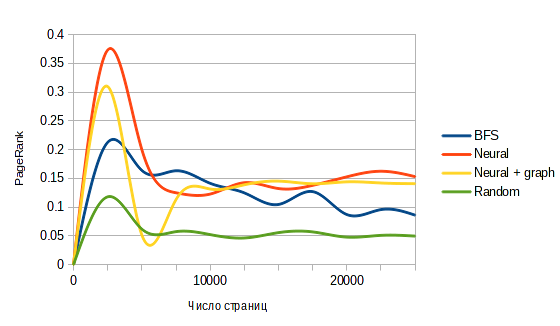
\includegraphics[width=1\linewidth]{pics/ranges5.png}}
\caption{График зависимости среднего $PageRank$ страниц от скачанного числа страниц. $BFS$ --- стратегия обхода в ширину. $Neural$ --- стратегия приоритезации, использующая нейронную сеть. $Neural + Graph$ --- стратегия приоритезации использующая нейронную сеть и веб-граф. $Random$ --- стратегия приоритезации, случайно выбирающая из коллекции страницу для скачивания.}
\label{graphic}
\end{figure}

Соответственно, стратегия тем лучше, чем выше $PageRank$ страниц, скачанных в процессе обхода интернета поисковым роботом, использующим ее, то есть, чем выше линия на графике.

\section{Выводы}

Полученные результаты экспериментального сравнения позволяют сделать следующие выводы:

\begin{enumerate}
\item Стратегия приоритезации, использующая метод обхода в ширину, превосходит стратегию, случайно выбирающую страницы.
\item Предложенные в работе стратегии приоритезации поискового робота, превосходят стандартную стратегию обхода в ширину.
\item Результаты обхода интернета с использованием двух предложенных стратегий отличаются незначительно.
\end{enumerate}

